%% Document template source: LaTeX2e template for FEUP's Project FE-UP
%% Document template author: jlopes@fe.up.pt
%% Template adapted

%% A alterar: <--ALTERAR-->

\documentclass[11pt,a4paper]{report}

%% Macros ----------------------------------------------------------------------
\newcommand{\school}{Instituto Superior de Engenharia de Lisboa}
\newcommand{\degree}{Licenciatura em Engenharia Eletrotécnica, Telecomunicações e Computadores}
\newcommand{\projisel}{Projeto ISEL 2023/24 --- LEETC}
\newcommand{\projtitle}{Computer Networks}
\newcommand{\projsubtitle}{Phase 4 - Deploy Services}
\newcommand{\projteam}{Grupo LP-07}

%% Package ---------------------------------------------------------------------
\usepackage[a4paper,left=25mm,right=25mm,top=25mm,bottom=25mm,headheight=6mm,footskip=12mm]{geometry}   % Document dimensions
\usepackage[T1]{fontenc}            % PS fonts
\usepackage[english]{babel}         % [portuges]??
\usepackage[export]{adjustbox}      %
\usepackage[normalem]{ulem}         % various types of underlining
\usepackage[table,xcdraw]{xcolor}   % driver-independent color extensions
\usepackage[utf8]{inputenc}         % accents
\usepackage{amsmath}                % multi-line and other mathematical statements
\usepackage{array}                  % Images in tables
\usepackage{booktabs}               %
\usepackage{caption}                % rotating captions, sideways captions, etc.
\usepackage{chicago}                % Bibliography style
\usepackage{color}                  %
\usepackage{fancyhdr}               % Headers and footers
\usepackage{float}                  % tables and figures in the multi-column environment 
\usepackage{graphicx}               % 
\usepackage{hyperref}               % Hyper references
\usepackage{lastpage}               % 
\usepackage{lipsum}                 % loren dummy text
\usepackage{listings}               % Programming syntax
\usepackage{longtable}              % Tables continue in the next page
\usepackage{multicol}               % 
\usepackage{multirow}               % tabular cells spanning multiple rows
\usepackage{newtxtext,newtxmath}    % do not use CM fonts
\usepackage{paralist}
\usepackage{setspace}               % setting the spacing between lines
\usepackage{subcaption}             % for subfigures and the like

%% Package settings ------------------------------------------------------------
\graphicspath{{./images}}                           % {graphicx} - Images path % BY PHASE!!!
\selectlanguage{english}                            % {babel} - Language portuguese
\setlength{\columnsep}{3cm}                         % {multicol} - Column spacement
\definecolor{engineering}{rgb}{0.549,0.176,0.098}   % {color}
\definecolor{cloudwhite}{cmyk}{0,0,0,0.025}         % {color}
\definecolor{deepblue}{rgb}{0,0,0.5}                % {color}
\definecolor{deepred}{rgb}{0.6,0,0}                 % {color}
\definecolor{deepgreen}{rgb}{0,0.5,0}               % {color}
\setlength{\parindent}{0em}                         % {geometry}
\setlength{\parskip}{1ex}                           % {geometry}
\lstdefinestyle{pythoncode}                         % {listings} - Python syntax
{
    aboveskip=8mm,
    backgroundcolor=\color{cloudwhite},             
    basicstyle=\footnotesize\ttfamily,
    numbers=left,                                   % where to put the line-numbers
    belowskip=4mm,
    breakatwhitespace=false,                        % sets if automatic breaks should only happen at whitespace
    breaklines=true,                                % sets automatic line breaking
    captionpos=b,                                   % sets the caption-position to bottom
    escapeinside={\%*}{*)},                         % if you want to add a comment within your code
    float=htb,
    frame=tb,
    keepspaces=true,
    keywordstyle=\bfseries\color{deepblue},
    morekeywords={*,var,template,new}               % if you want to add more keywords to the set
    numbersep=8pt,                                  % how far the line-numbers are from the code
    numberstyle=\scriptsize\texttt,                 % the size of the fonts that are used for the line-numbers
    showspaces=false,                               % show spaces adding particular underscores
    showstringspaces=false,                         % underline spaces within strings
    showtabs=false,                                 % show tabs within strings adding particular underscores
    stepnumber=1,                                   % the step between two line-numbers. If it's 1 each line will be numbered
    stringstyle=\color{deepgreen},
    tabsize=2,                                      % sets default tabsize to 2 spaces
}
\lstdefinestyle{termoutputs}                        % {listings} - Python syntax
{
    aboveskip=8mm,
    backgroundcolor=\color{cloudwhite},             
    basicstyle=\scriptsize\ttfamily,
    numbers=left,                                   % where to put the line-numbers
    belowskip=4mm,
    breakatwhitespace=false,                        % sets if automatic breaks should only happen at whitespace
    breaklines=true,                                % sets automatic line breaking
    captionpos=b,                                   % sets the caption-position to bottom
    escapeinside={\%*}{*)},                         % if you want to add a comment within your code
    float=htb,
    frame=tb,
    keepspaces=true,
    keywordstyle=\bfseries\color{deepblue},
    morekeywords={*,var,template,new}               % if you want to add more keywords to the set
    numbersep=8pt,                                  % how far the line-numbers are from the code
    numberstyle=\scriptsize\texttt,                 % the size of the fonts that are used for the line-numbers
    showspaces=false,                               % show spaces adding particular underscores
    showstringspaces=false,                         % underline spaces within strings
    showtabs=false,                                 % show tabs within strings adding particular underscores
    stepnumber=1,                                   % the step between two line-numbers. If it's 1 each line will be numbered
    stringstyle=\color{deepgreen},
    tabsize=2,                                      % sets default tabsize to 2 spaces
}
\fancyhf{}                                          % {fancyhdr} clear off all default fancyhdr headers and footers
\lfoot{\small{\emph{\projtitle, \projsubtitle}}}    % {fancyhdr}
\rfoot{\small{\thepage\ / \pageref{LastPage}}}      % {fancyhdr}
\pagestyle{fancy}                                   % {fancyhdr} apply the fancy header style
\renewcommand{\headrulewidth}{0.0pt}                % {fancyhdr} no head rule
\renewcommand{\footrulewidth}{0.4pt}                % {fancyhdr}
\hypersetup{                                        % {hyperref}
    plainpages=false,
    pdfpagelayout=SinglePage,
    bookmarksopen=false,
    bookmarksnumbered=true,
    breaklinks=true,
    linktocpage,
    colorlinks=true,
    linkcolor=engineering,
    urlcolor=engineering,
    filecolor=engineering,
    citecolor=engineering,
    allcolors=engineering
}

%% Document start --------------------------------------------------------------
\begin{document}
    \pagenumbering{roman}\setcounter{page}{1}

%% Cover -----------------------------------------------------------------------
\begin{titlepage}
    \center

    \vspace*{-12mm}
    {\large \textbf{\textsc{\school}}}\\

    \vfill

    
\includegraphics[width=62mm]{logoisel}
    
    \vfill
    
    {\huge \textbf{\projtitle}}\\[6mm]
    {\Large \textbf{\projsubtitle}}\\
    
    \vfill
    
    \vfill
    
    {\Large \textbf{\projisel}}\\[12mm]
    
    {\Large \textbf{Coordination}}\\[4mm]
    {\large General: Carlos Meneses\hspace*{18mm}
            Course: Nuno Cruz}\\[6mm]
    
    {\Large \textbf{\projteam}}\\[4mm]
    {\large Supervisor: Luís Pires\hspace*{12mm}}\\[6mm]
    
    {\Large \textbf{Student}}\\[4mm]
    {\large Nuno Brito $<$A46948@alunos.isel.pt$>$}
    
    \vspace*{10mm}
    
    \renewcommand{\today}{June 2th 2024}
    \today
    
\end{titlepage}

%% TOC -------------------------------------------------------------------------
\tableofcontents

%% List of figures -------------------------------------------------------------
\listoffigures
\addcontentsline{toc}{chapter}{Figure list}

%% List of tables --------------------------------------------------------------
\listoftables
\addcontentsline{toc}{chapter}{Table list}

%% List of listings --------------------------------------------------------------
\lstlistoflistings
\addcontentsline{toc}{chapter}{Listings list}

%% Acronyms --------------------------------------------------------------------
\chapter*{Acronyms list}
    \addcontentsline{toc}{chapter}{Acronyms list}

    \begin{flushleft}
        \begin{tabular}{l p{0.8\linewidth}}
            API     & Application Programming Interface\\
            CLI     & Command Line Interface\\
            CMD     & Command Prompt\\
            DHCP    & Dynamic Host Configuration Protocol\\
            DNS     & Domain Name System\\
            GUI     & Graphical User Interface\\
            HTTP    & Hyper Text Transfer Protocol\\
            HTTPS   & Hyper Text Transfer Protocol Secure\\
            IP      & Internet Protocol\\
            IPv4    & Internet Protocol version 4\\
            IPv6    & Internet Protocol version 6\\
            LAN     & Local Area Network\\
            OS      & Operating System\\
            OSS     & openSUSE\\
            OSI     & Open Systems Interconnection\\
            PC      & Personal Computer\\
            PHP     & PHP: Hypertext Preprocessor\\
            SSL     & Secure Sockets Layer\\
            TCP     & Transmission Control Protocol\\
            TLS     & Transport Layer Security\\
            TUI     & Terminal User Interface\\ % Not used yet
            UDP     & User Datagram Protocol\\
            VPN     & Virtual Private Network\\
            WWW     & World Wide Web\\
            XAMPP   & Cross-Platform, Apache, MySQL, PHP, and Perl
        \end{tabular}
    \end{flushleft}

%% Glossary --------------------------------------------------------------------
\chapter*{Glossary}
    \addcontentsline{toc}{chapter}{Glossary}

    \begin{description}
        \item[Apache2] \hfill \\
            An opensource HTTP web server.
        \item[Bit] \hfill \\
            A unit of information in computing and digital communications. The bit represents a logical state with one of two possible values, 0 or 1 (other representations such as \textit{true / false} are also valid).
        \item[Byte] \hfill \\
            Also a unit of digital information, consists of 8 bits.
        \item[Broadcast] \hfill \\
            A method of transferring a message to all recipients simultaneously.
        \item[Browser] \hfill \\
            A browser is a internet navigation software. It comes in multiple flavours, nowadays the big three are Microsoft Edge, Mozilla Firefox and Google Chrome.
        \item[Cisco Packet Tracer] \hfill \\
            A cross-platform visual network simulation tool.
        \item[Command Prompt] \hfill \\
            The default command-line interpreter for Windows operating systems.
        \item[Firewall] \hfill \\
            A barrier between networks. Controls inbound and outbound traffic.
        \item[Gateway] \hfill \\
            A network gateway provides a connection between networks and devices. Known as protocol translation gateways or mapping gateways, can perform protocol conversions to connect networks with different network protocol technologies.
        \item[LibreWolf] \hfill \\
            An internet browser based on Mozilla's Firefox. It's primary purpose is to allow privacy, and with it comes security. It achieves this by removing telemetry and data collection.
        \item[Linux] \hfill \\
            Open-source Unix-like operating systems based on the Linux kernel.
        \item[MariaDB] \hfill \\
            A community-developed fork of MySQL database server.
        \item[openSUSE Tumbleweed] \hfill \\
            An openSUSE (OSS) is an open-source community driven Linux-based distribuition sponsored by SUSE Software Solutions. Tumbleweed is a rolling release version allowing for up-to-date software releases.
        \item[Operating system] \hfill \\
            A program that manages a computer's resources from software to hardware.
        \item[Ping] \hfill \\
             A software utility used to test the reachability of a host on an IP network.
        \item[Tracert] \hfill \\
            Or \textbf{traceroute} in unix and linux systems, is a computer network diagnostic command for displaying possible routes and measuring transit delays of packets across an IP network.
        \item[Ipconfig] \hfill \\
            Or \textbf{ifconfig} in unix and linux systems, is a console application program that displays all current TCP/IP network configuration values.
        \item[Python] \hfill \\
            Python is a high-level programming language, object-oriented.
        \item[Perl] \hfill \\
            A high-level, general-purpose, interpreted, dynamic programming language
        \item[Rolling release distribuition] \hfill \\
            A distribuition where it's software release cycle is more frequent than those of Long Term Support (LTS). It's up to the Linux-based distribuitor to guarantee the testing of a package.
        \item[Router] \hfill \\
            A networking device that forwards data packets between computer networks, including internetworks such as the global Internet.
        \item[Switch] \hfill \\
            A networking hardware that connects devices on a computer network by using packet switching to receive and forward data to the destination device.
        \item[Socket] \hfill \\
            A network socket serves as an endpoint for sending and receiving data across the network.
        \item[Subnet Mask] \hfill \\
            Is a logical subdivision of an IP network.
        \item[Unix] \hfill \\
            Is a family of multitasking, multi-user computer operating systems that derive from the original AT\&T Unix.
        \item[VPN] \hfill \\
            A private network creating a secure connection between a device and a network.
        \item[Windows] \hfill \\
            Microsoft's operating system. First released in 1985 as a Graphical User Interface (GUI) for MS-DOS, continued to evolve with it's latest version being 11.
            Due to it's nature, it's not recommended for server production environment.
        \item[Wireshark] \hfill \\
            Wireshark is a network protocol analyser software. Allows traffic capture between a computer and a network.
        \item[XAMPP] \hfill \\
            A software package environment collection containing Apache2 webserver, MariaDB database, PHP and Perl.
    \end{description}

%% Chapter: introduction -------------------------------------------------------
\chapter{Introduction}
% display headers & footers
    \pagestyle{fancy}
    We've reached our big finale. In phase 4 we'll accomplish a network managed by a DHCP server, web surf to an HTTP server and use a DNS to recognize a web page by name.\\
    Applying everything learned until now and much more.

% main page numbers with arabic numerals
    \pagenumbering{arabic}\setcounter{page}{1}

%% Chapter: phase 4 ------------------------------------------------------------
\chapter{Phase 4}
    \section{Tehcnical aspects}
        For phase 4 there's going to be some recycling.\\
        Mathematical formulas:
        \[
            Clients_{LAN_A} = max\left(20, \left(\sum_{k=0}^n studentnumber_k\right)mod 100\right)\quad <=> 
            Clients_{LAN_A} = 48\quad
        \] \\
        \[
            Clients_{LAN_B} = \frac{Clients_{LAN_A}}{2}\quad <=>
            Clients_{LAN_B} = 27\quad
        \]\\

        Static routes:
        \begin{longtable}[c]{@{}lllllclc@{}}
        \toprule
            \textbf{Router}     & \textbf{From}                  & \textbf{To} & \textbf{Network} & \textbf{Via}                                       & \multicolumn{3}{c}{\textbf{Through}}                                        \\* \midrule
            \endfirsthead
            %
            \multicolumn{8}{c}%
            {{\bfseries Table \thetable\ continued from previous page}} \\
            \toprule
            \textbf{Router}     & \textbf{From}                  & \textbf{To} & \textbf{Network} & \textbf{Via}                                       & \multicolumn{3}{c}{\textbf{Through}}                                        \\* \midrule
            \endhead
            %
            \multirow{2}{*}{R1} & \multirow{2}{*}{LAN A / LAN B} & LAN Servers & 192.168.7.0/25   & 192.168.7.254                                      & \multirow{2}{*}{R1} & \textgreater{}                  & R2                  \\
                                &                                & Any         & 8.8.8.8/30       & 192.168.7.249                                      &                     & \textgreater{}                  & R0                  \\* \midrule
            \multirow{3}{*}{R2} & \multirow{3}{*}{LAN Servers}   & LAN A       & 192.168.7.128/26 & \multicolumn{1}{c}{\multirow{2}{*}{192.168.7.253}} & \multirow{3}{*}{R2} & \multirow{2}{*}{\textgreater{}} & \multirow{2}{*}{R1} \\
                                &                                & LAN B       & 192.168.7.192/27 & \multicolumn{1}{c}{}                               &                     &                                 &                     \\* \cmidrule(lr){3-5} \cmidrule(l){7-8}
                                &                                & Any         & 8.8.8.8/30       & 192.168.7.245                                      &                     & \textgreater{}                  & R0                  \\* \midrule
            \multirow{3}{*}{R0} & \multirow{3}{*}{Any}           & LAN A       & 192.168.7.128/26 & \multicolumn{1}{c}{\multirow{2}{*}{192.168.7.250}} & \multirow{3}{*}{R0} & \multirow{2}{*}{\textgreater{}} & \multirow{2}{*}{R1} \\
                                &                                & LAN B       & 192.168.7.192/27 & \multicolumn{1}{c}{}                               &                     &                                 &                     \\* \cmidrule(lr){3-5} \cmidrule(l){7-8}
                                &                                & LAN Servers & 192.168.7.0/25   & 192.168.7.246                                      &                     & \textgreater{}                  & R2                  \\* \bottomrule
            \caption{Static routes table}
            \label{tab:staticroutetbl}\\
        \end{longtable}

        IP allocation:
        \begin{longtable}[c]{lllllll}
            \hline
                                                                                                  & \textbf{Network}            & \textbf{Usable IPs} & \textbf{Router} & \textbf{Broadcast} & \multicolumn{1}{c}{\textbf{Subnet Mask}} &                                      \\ \cline{2-5}
            \multirow{-2}{*}{\textbf{Name}}                                                       & \multicolumn{4}{c}{192.168.7.}                                                           & \multicolumn{1}{c}{255.255.255.}         & \multirow{-2}{*}{\textbf{Populated}} \\ \hline
            \endfirsthead
            %
            \multicolumn{7}{c}%
            {{\bfseries Table \thetable\ continued from previous page}} \\
            \hline
                                                                                                  & \textbf{Network}            & \textbf{Usable IPs} & \textbf{Router} & \textbf{Broadcast} & \multicolumn{1}{c}{\textbf{Subnet Mask}} &                                      \\ \cline{2-5}
            \multirow{-2}{*}{\textbf{Name}}                                                       & \multicolumn{4}{c}{192.168.7.}                                                           & \multicolumn{1}{c}{255.255.255.}         & \multirow{-2}{*}{\textbf{Populated}} \\ \hline
            \endhead
            %
            \hline
            \endfoot
            %
            \endlastfoot
            %
            \cellcolor[HTML]{F4B084}\textbf{LAN Server}                                           & 0                           & 1 - 125             & 126             & 127                & 128                                      & 126                                  \\
            \cellcolor[HTML]{A9D08E}\textbf{LAN A}                                                & 128                         & 129 - 189           & 190             & 191                & 192                                      & 48                                   \\
            \cellcolor[HTML]{FFD966}\textbf{LAN B}                                                & 192                         & 193 - 221           & 222             & 223                & 224                                      & 27                                   \\ \hline
            \multirow{+2}{*}{\textbf{\begin{tabular}[c]{@{}l@{}}Unused\\ remaining\end{tabular}}} & \cellcolor[HTML]{BFBFBF}224 & 225 - 238           &                 & 239                &                                          & 0                                    \\
                                                                                                  & \cellcolor[HTML]{C09FE5}240 & 241 - 242           &                 & 243                &                                          & 0                                    \\ \hline
            \cellcolor[HTML]{C09FE5}\textbf{LAN Transit C}                                        & 244                         & 245 - 246           &                 & 247                & 252                                      & 2                                    \\
            \cellcolor[HTML]{C09FE5}\textbf{LAN Transit B}                                        & 248                         & 249 - 250           &                 & 251                & 252                                      & 2                                    \\
            \cellcolor[HTML]{C09FE5}\textbf{LAN Transit A}                                        & 252                         & 253 - 254           &                 & 255                & 252                                      & 2                                    \\ \hline
            \caption{LAN allocation table}
            \label{tab:lanalloctable}\\
        \end{longtable}

        But we also have new toys to play with.\\

        A fully functional DHCP server capable of assigning IP addresses to LAN's A and B.\\
        But how does it work? Well, for starters it works in the application layer (7) of the Open Systems Interconnection (OSI) model. A plot twist for sure as it could be easily mistaken for a network layer. It uses UDP protocol for its connectionless model and operates in four phases (no pun intended): server discovery, IP lease offer, IP lease request, and IP lease acknowledgement.\\

        "BUT WAIT, there's more!" Since our DHCP server is located in another subnetwork and behind another router, we must somehow be able to \textbf{\textit{relay}} the assigned IP address to our devices in LAN's A and B. So that's exactly what we are going to create, a relay. In the following sections a detailed explained will be presented.\\

        Additionally a web server will also be deployed to serve a single web page. To reach it like a sanely human being a Domain Name Service (DNS) record will also be created.\\
        A DNS is a hierarchical and distributed name service that provides a naming system for computers and other services. There's all types of records: MX for SMTP mail exchangers, NS for name servers, PTR for pointers for reverse DNS lookups, CNAME for domain name aliases and A and AAAA for IP addresses. For this project it's the latter one we're using.

    \section{Changes}
        For this phase we are reverting some configurations, namely LAN's A and B devices static IP address. \\
        The rest are still valid here, now as IP pool addresses.
        \begin{longtable}[c]{llrllrr}
            \hline
            \multicolumn{1}{c}{\multirow{3}{*}{\textbf{Name}}} & \multicolumn{2}{c}{\multirow{2}{*}{\textbf{Ports Link}}} & \multicolumn{1}{c}{\multirow{3}{*}{\textbf{Network}}} & \multicolumn{1}{c}{\multirow{2}{*}{\textbf{IP}}} & \multicolumn{1}{c}{\multirow{2}{*}{\textbf{Gateway}}} & \multicolumn{1}{c}{\multirow{2}{*}{\textbf{Subnet Mask}}} \\
            \multicolumn{1}{c}{}                               & \multicolumn{2}{c}{}                                     & \multicolumn{1}{c}{}                                  & \multicolumn{1}{c}{}                             & \multicolumn{1}{c}{}                                  & \multicolumn{1}{c}{}                                      \\ \cline{2-3} \cline{5-7}
            \multicolumn{1}{c}{}                               & \textbf{From}                & \textbf{To}               & \multicolumn{1}{c}{}                                  & \multicolumn{2}{c}{192.168.7.}                                                                           & \multicolumn{1}{c}{255.255.255.}                          \\ \hline
            \endfirsthead
            %
            \multicolumn{7}{c}%
            {{\bfseries Table \thetable\ continued from previous page}} \\
            \hline
            \multicolumn{1}{c}{\multirow{3}{*}{\textbf{Name}}} & \multicolumn{2}{c}{\multirow{2}{*}{\textbf{Ports Link}}} & \multicolumn{1}{c}{\multirow{3}{*}{\textbf{Network}}} & \multicolumn{1}{c}{\multirow{2}{*}{\textbf{IP}}} & \multicolumn{1}{c}{\multirow{2}{*}{\textbf{Gateway}}} & \multicolumn{1}{c}{\multirow{2}{*}{\textbf{Subnet Mask}}} \\
            \multicolumn{1}{c}{}                               & \multicolumn{2}{c}{}                                     & \multicolumn{1}{c}{}                                  & \multicolumn{1}{c}{}                             & \multicolumn{1}{c}{}                                  & \multicolumn{1}{c}{}                                      \\ \cline{2-3} \cline{5-7}
            \multicolumn{1}{c}{}                               & \textbf{From}                & \textbf{To}               & \multicolumn{1}{c}{}                                  & \multicolumn{2}{c}{192.168.7.}                                                                           & \multicolumn{1}{c}{255.255.255.}                          \\ \hline
            \endhead
            %
            \hline
            \endfoot
            %
            \endlastfoot
            %
            \textbf{PC0}                                       & Fa0                          & Sw0 Fa0/2                 & \multirow{2}{*}{LAN A}                                & \multicolumn{2}{l}{\multirow{2}{*}{}}                                                                    & \multirow{2}{*}{192}                                      \\
            \textbf{Laptop0}                                   & Fa0                          & Sw0 Fa0/3                 &                                                       & \multicolumn{2}{l}{}                                                                                     &                                                           \\ \hline
            \textbf{PC1}                                       & Fa0                          & Sw1 Fa0/2                 & \multirow{2}{*}{LAN B}                                & \multicolumn{2}{l}{\multirow{2}{*}{}}                                                                    & \multirow{2}{*}{224}                                      \\
            \textbf{Laptop1}                                   & Fa0                          & Sw1 Fa0/3                 &                                                       & \multicolumn{2}{l}{}                                                                                     &                                                           \\ \hline
            \multirow{3}{*}{\textbf{R0}}                       & Fa0/0                        & Fa0/0                     & External                                              &                                                  &                                                       & \multicolumn{1}{l}{}                                      \\ \cline{5-7}
                                                               & Fa4/0                        & R2 Fa4/0                  & LAN Transit C                                         & 245                                              &                                                       & \multirow{2}{*}{252}                                      \\
                                                               & Fa5/0                        & R1 Fa5/0                  & LAN Transit B                                         & 249                                              &                                                       &                                                           \\ \hline
            \multirow{4}{*}{\textbf{R1}}                       & Fa0/0                        & Sw0 Fa0/1                 & LAN A                                                 & 190                                              &                                                       & 192                                                       \\
                                                               & Fa1/0                        & Sw1 Fa0/1                 & LAN B                                                 & 222                                              &                                                       & 224                                                       \\ \cline{5-7}
                                                               & Fa4/0                        & R2 Fa5/0                  & LAN Transit A                                         & 253                                              &                                                       & \multirow{2}{*}{252}                                      \\
                                                               & Fa5/0                        & R1 Fa4/0                  & LAN Transit B                                         & 250                                              &                                                       &                                                           \\ \hline
            \multirow{3}{*}{\textbf{R2}}                       & Fa0/0                        & Sw2 Fa0/4                 & LAN Server                                            & 126                                              &                                                       & 128                                                       \\ \cline{5-7}
                                                               & Fa4/0                        & R0 Fa4/0                  & LAN Transit C                                         & 246                                              &                                                       & \multirow{2}{*}{252}                                      \\
                                                               & Fa5/0                        & R1 Fa4/0                  & LAN Transit A                                         & 254                                              &                                                       &                                                           \\ \hline
            \textbf{HTTP-Server}                               & Fa0                          & Sw2 Fa0/1                 & \multirow{3}{*}{LAN Server}                           & 3                                                & \multirow{3}{*}{126}                                  & \multirow{3}{*}{128}                                      \\
            \textbf{DNS-Server}                                & Fa0                          & Sw2 Fa0/2                 &                                                       & 2                                                &                                                       &                                                           \\
            \textbf{DHCP-Server}                               & Fa0                          & Sw2 Fa0/3                 &                                                       & 1                                                &                                                       &                                                           \\ \hline
            \multirow{3}{*}{\textbf{Sw0}}                      & Fa0/1                        & R1 Fa0/0                  & \multirow{3}{*}{LAN A}                                & \multicolumn{3}{c}{\multirow{3}{*}{}}                                                                                                                                \\
                                                               & Fa0/2                        & PC0                       &                                                       & \multicolumn{3}{c}{}                                                                                                                                                 \\
                                                               & Fa0/3                        & Laptop0                   &                                                       & \multicolumn{3}{c}{}                                                                                                                                                 \\ \hline
            \multirow{3}{*}{\textbf{Sw1}}                      & Fa0/1                        & R1 Fa1/0                  & \multirow{3}{*}{LAN B}                                & \multicolumn{3}{c}{\multirow{3}{*}{}}                                                                                                                                \\
                                                               & Fa0/2                        & PC1                       &                                                       & \multicolumn{3}{c}{}                                                                                                                                                 \\
                                                               & Fa0/3                        & Laptop1                   &                                                       & \multicolumn{3}{c}{}                                                                                                                                                 \\ \hline
            \multirow{4}{*}{\textbf{Sw2}}                      & Fa0/1                        & HTTP-Server               & \multirow{4}{*}{LAN Server}                           & \multicolumn{3}{c}{\multirow{4}{*}{}}                                                                                                                                \\
                                                               & Fa0/2                        & DNS-Server                &                                                       & \multicolumn{3}{c}{}                                                                                                                                                 \\
                                                               & Fa0/3                        & DHCP-Server               &                                                       & \multicolumn{3}{c}{}                                                                                                                                                 \\
                                                               & Fa0/4                        & R2 Fa0/0                  &                                                       & \multicolumn{3}{c}{}                                                                                                                                                 \\ \hline
            \caption{IP configuration table}
            \label{tab:ipconftable}\\
        \end{longtable}

    \section{Server configuration}
        Servers should be configured with static IP addresses, either in the device itself of in a network controller.
        \begin{figure}[h]
            \centering
            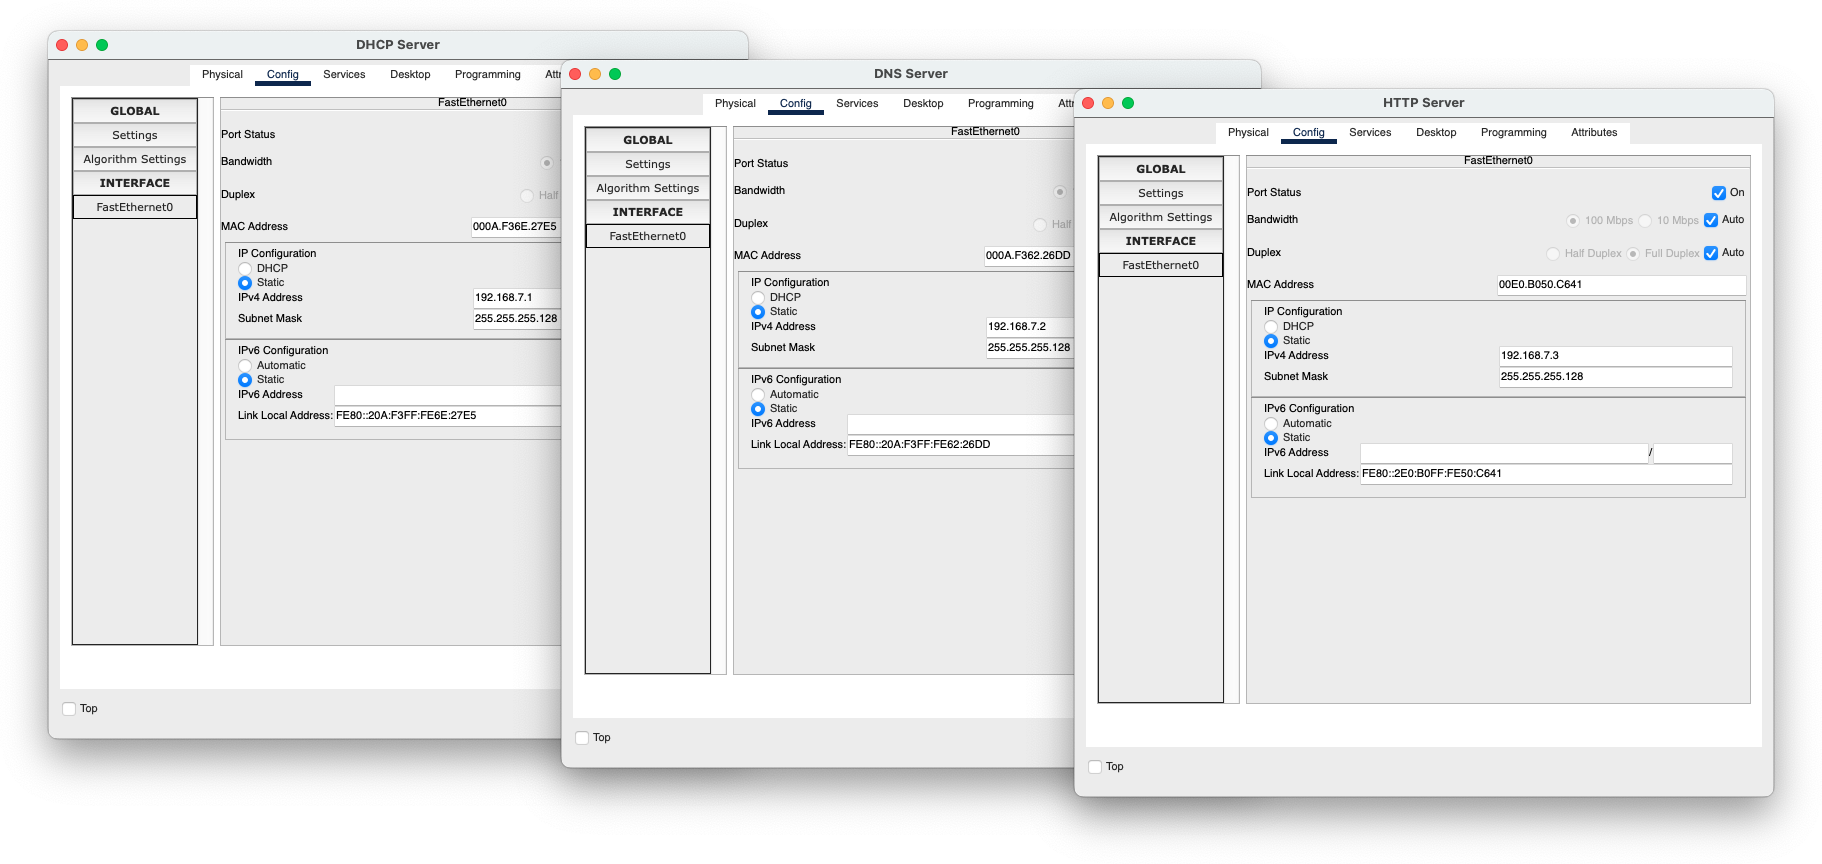
\includegraphics[scale=0.25]{LanServer-IP}
            \caption{LanServer devices static IP addresses}
            \label{tab:lanserverdev}
        \end{figure}

        Using our reference table, we proceed with the pool assignment.
        \begin{figure}[h]
            \centering
            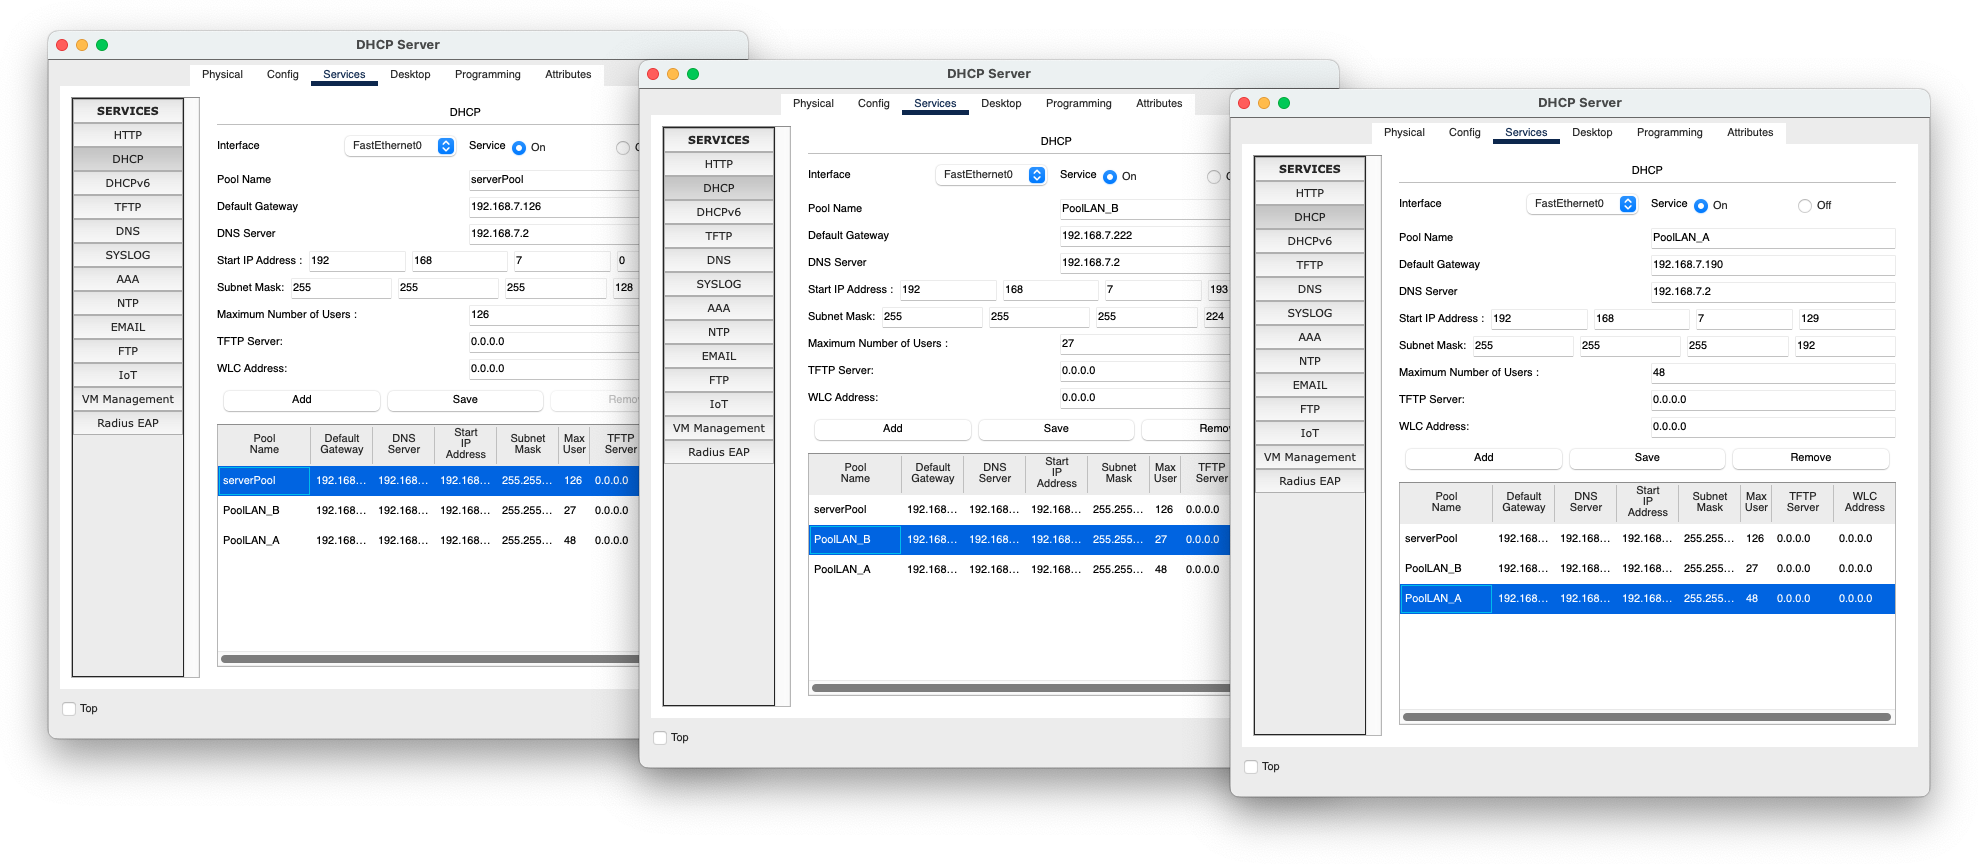
\includegraphics[scale=0.23]{DHCP-Pool}
            \caption{DHCP pool configuration}
            \label{tab:dhcpconf}
        \end{figure}

        To allow access to our HTTP server using a name and not a prisioner number we must configure a record. In this case, as refered before, A record.
        \begin{figure}[h]
            \centering
            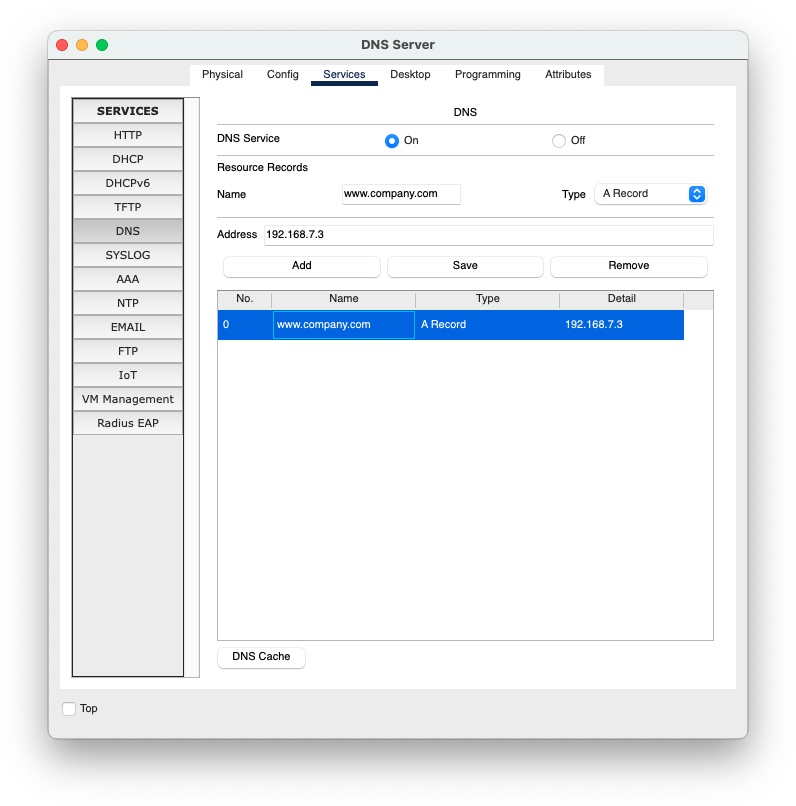
\includegraphics[scale=0.35]{DNS-Record}
            \caption{DNS records configuration}
            \label{tab:dnsconf}
        \end{figure}

    \section{Router additional configuration}
        Router 1 needs a tiny little command to allow our DHCP server: ip helper-address \textbf{\textit{DHCP.IP.ADDRESS}}\\
        Simple as that.
        \begin{figure}[h]
            \centering
            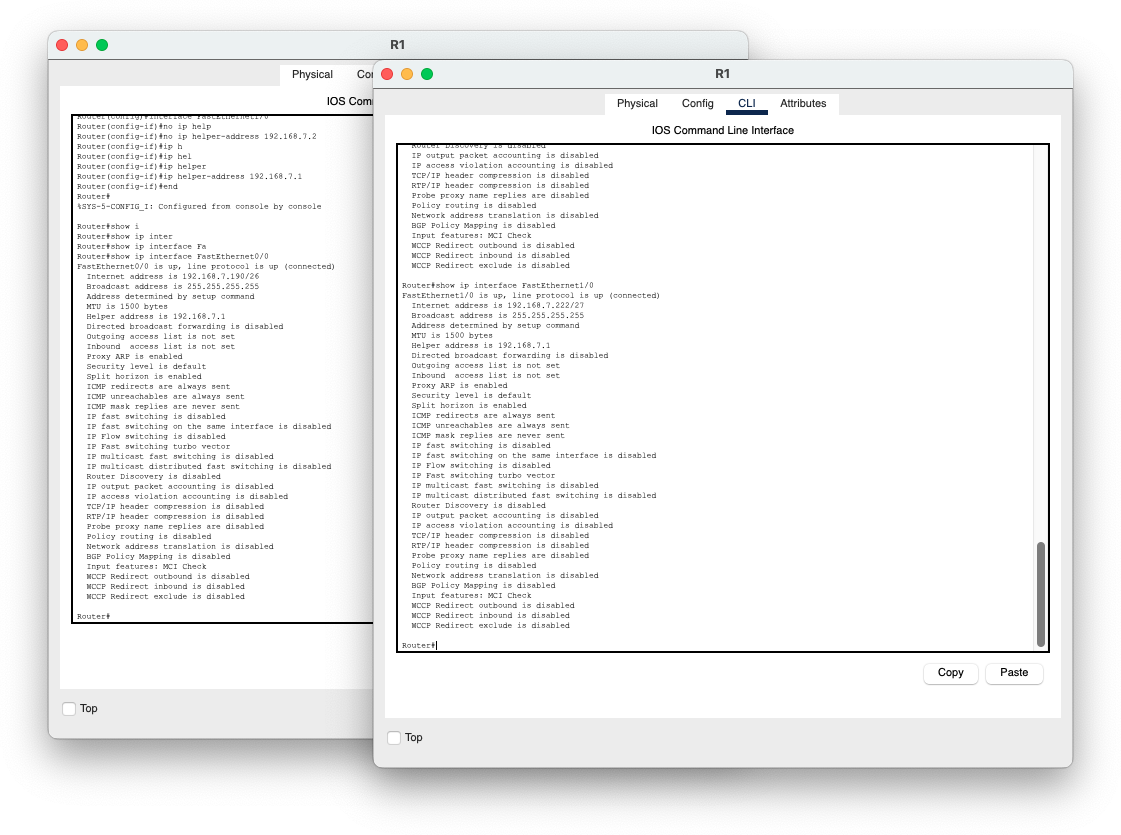
\includegraphics[scale=0.40]{R1}
            \caption{Router1 helper-address}
            \label{tab:router1}
        \end{figure}

    \section{Preparing devices and results}
        For our devices we'll configure them as DHCP. What follows are the executed commands.\\

        With PC0 we went above and beyond testing the network. First observing the new assigned IP by our DHCP server, then running nslookup to the HTTP server configured website and, to conclude, IP address renewal.\\
        We can also see the browser in action, showing that everything is working as expected.\\

        The remaining devices are in the \ref{printscreens} section from the appendix \ref{appendixref}.

        \begin{figure}[h]
            \centering
            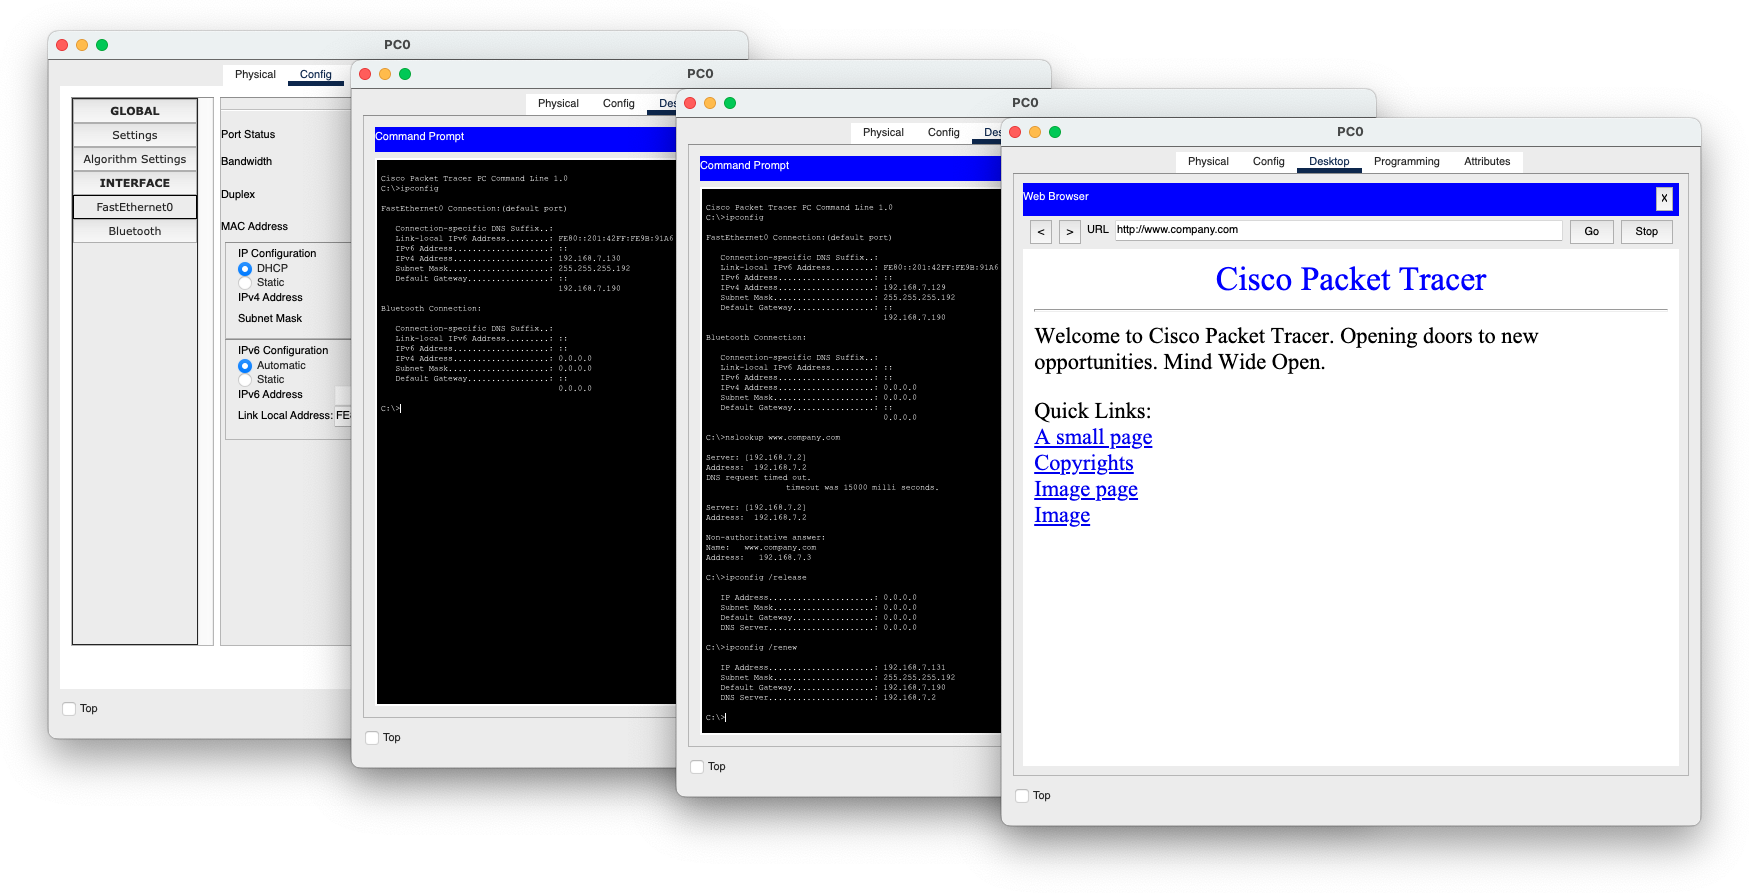
\includegraphics[scale=0.26]{PC0}
            \caption{PC0 configuration and commands}
            \label{tab:pc0conf}
        \end{figure}

        \pagebreak

    \section{Command line outputs}
        \lstset{style=termoutputs}
        \lstinputlisting[
            language={},
            caption={PC0 output (LAN A)},
            label={lst:pc0output}
        ]{./outputs/PC0.txt}

        \lstinputlisting[
            language={},
            caption={PC1 output (LAN B)},
            label={lst:pc1output}
        ]{./outputs/PC1.txt}

        \lstinputlisting[
            language={},
            caption={R1 output},
            label={lst:r1output}
        ]{./outputs/R1.txt}

        The remaining devices are in the \ref{clioutapxref} section from the appendix \ref{appendixref}.

%% Chapter: issues and fixes ---------------------------------------------------
\chapter{Issues and fixes}
    \textbf{Cisco Packet Tracer in MacOS:}\\
        \hspace*{10mm}*STILL* no solution was found to deal with those annoying popups that takes primary focus over other windows, even using the latest version.\\

%% Chapter: conclusions --------------------------------------------------------
\chapter{Conclusions}
    Looking at our output results we realize that everything is working as anticipated.\\
    We have IP addresses being assigned by a DHCP server over different sub networks and behind multiple routers. Renewal requests by devices are served without trouble.\\
    DNS records are also fully functional, devices can reach the web server by name and IP address. Unfortunately the same cannot be done for DHCP assigned IP addresses, only static addresses.

%% Bibliography ----------------------------------------------------------------
%\renewcommand{\bibname}{Bibliographic references}
%\bibliographystyle{chicago}
%\bibliography{refs}
%\addcontentsline{toc}{chapter}{\refname}  % add it to table of contents

%% Appendix --------------------------------------------------------------------
\appendix
    \chapter{Outputs}
    \label{appendixref}
        \section{Command line encore}
        \label{clioutapxref}

        \lstset{style=termoutputs}
        \lstinputlisting[
            language={},
            caption={Laptop0 output (LAN A)},
            label={lst:laptop0output}
        ]{./outputs/Laptop0.txt}
        \lstinputlisting[
            language={},
            caption={Laptop1 output (LAN B)},
            label={lst:laptop1output}
        ]{./outputs/Laptop1.txt}

    \chapter{Remaining devices}
        \section{Printscreens}
        \label{printscreens}

        \begin{figure}[h]
            \centering
            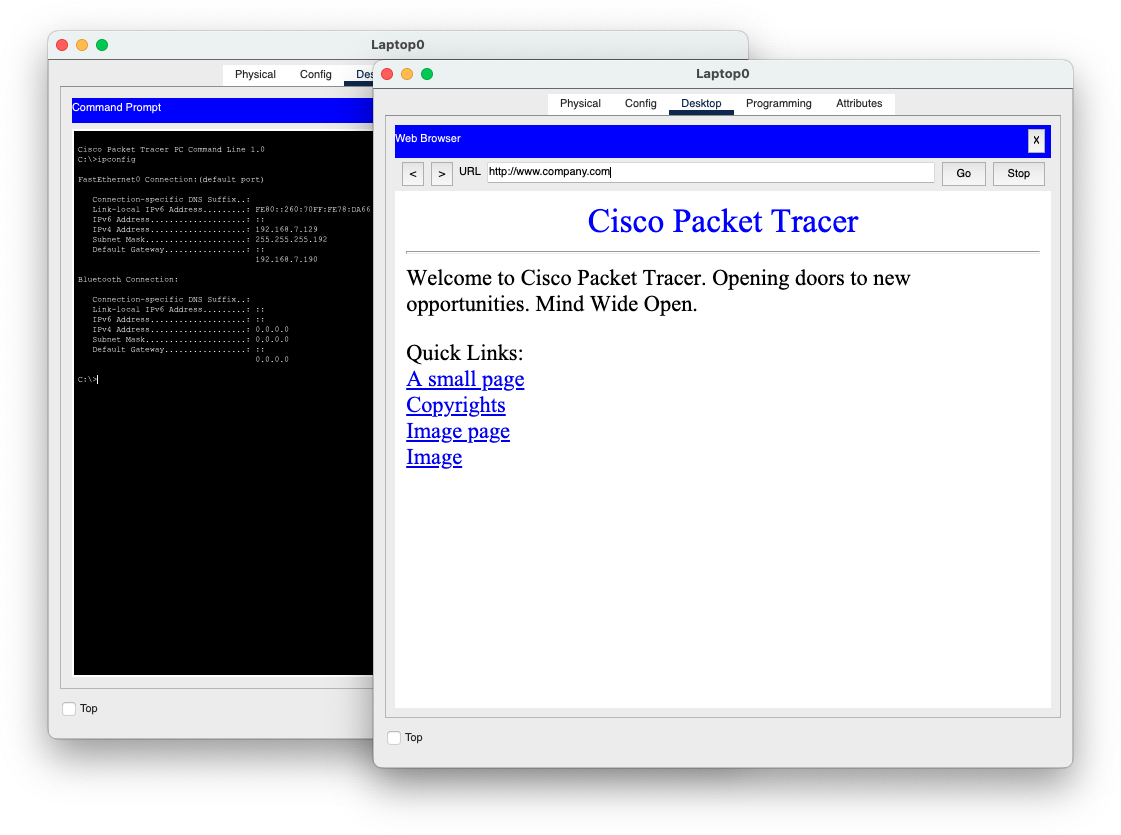
\includegraphics[scale=0.40]{Laptop0}
            \caption{Laptop0 configuration and commands}
            \label{tab:laptop0conf}
        \end{figure}

        \begin{figure}[h]
            \centering
            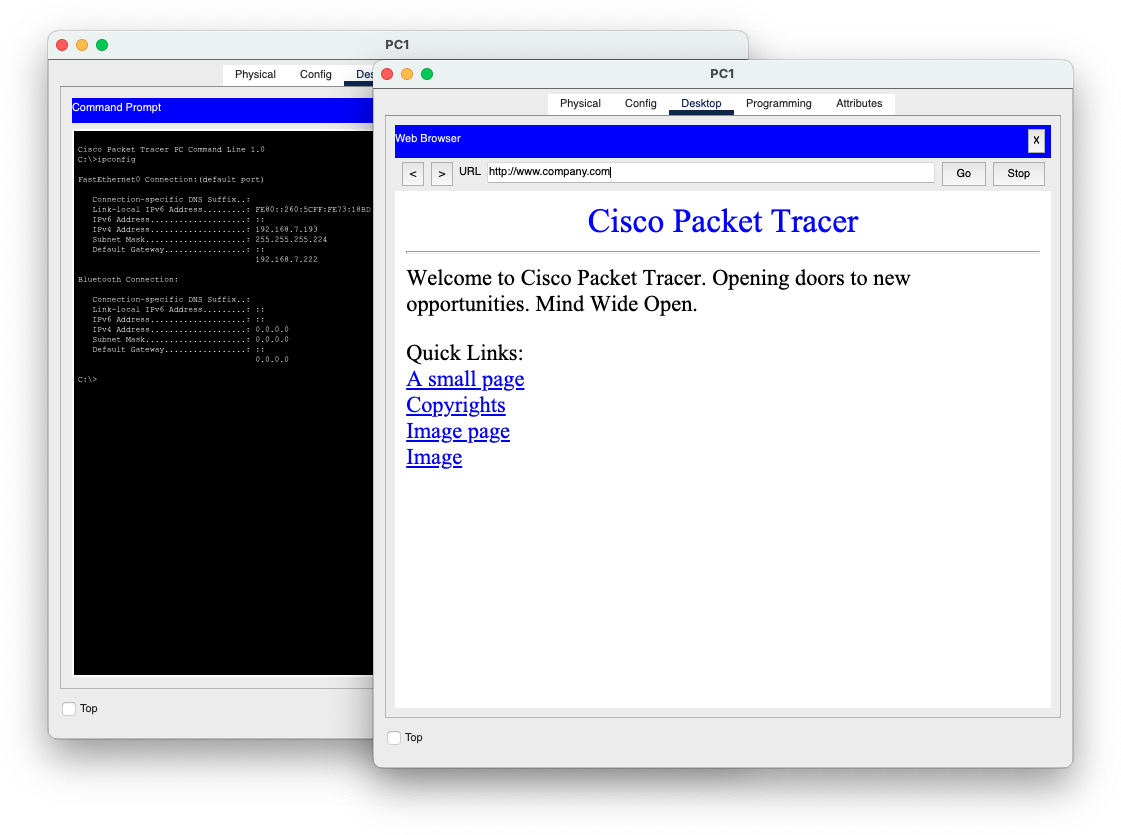
\includegraphics[scale=0.40]{PC1}
            \caption{PC1 configuration and commands}
            \label{tab:pc1conf}
        \end{figure}

        \begin{figure}[h]
            \centering
            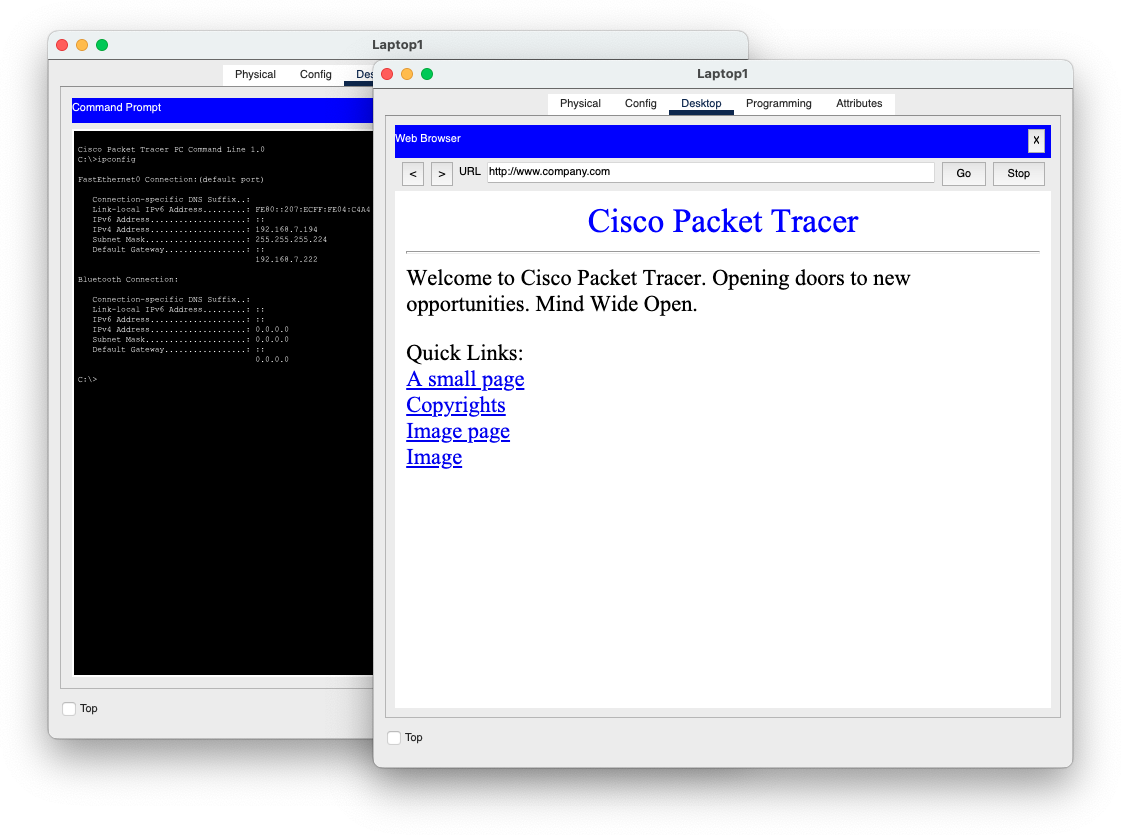
\includegraphics[scale=0.40]{Laptop1}
            \caption{Laptop1 configuration and commands}
            \label{tab:laptop1conf}
        \end{figure}

\end{document}
